\chapter{$b\bar{b}$-tagging Scale Factors for W jets in $t\bar{t}$ Events}

Boosted W bosons can arise in many models of beyond the SM physics. The 67.41\% branching fraction of $\textrm{W} \rightarrow \textrm{hadrons}$ make their reconstruction as AK8 jets an efficient channel. Although W bosons do not decay to b-quarks (the top quark is too heavy), the $b\bar{b}$-tagger has a non-zero probability to tag one of these jets as having decayed to a $b\bar{b}$ pair. This \textit{mistag} rate can, in principle, be different in simulation compared to in data. Depending on the use, it may be necessary to apply \textit{scale factors} to the simulation to correct for this difference. By using a sample of AK8 jets identified as W bosons in semi-leptonic $t\bar{t}$ events, we can calculate the mistag rate in both data and simulation, taking their ratio to form the scale factors.

\begin{figure}[hbp!]
\centering
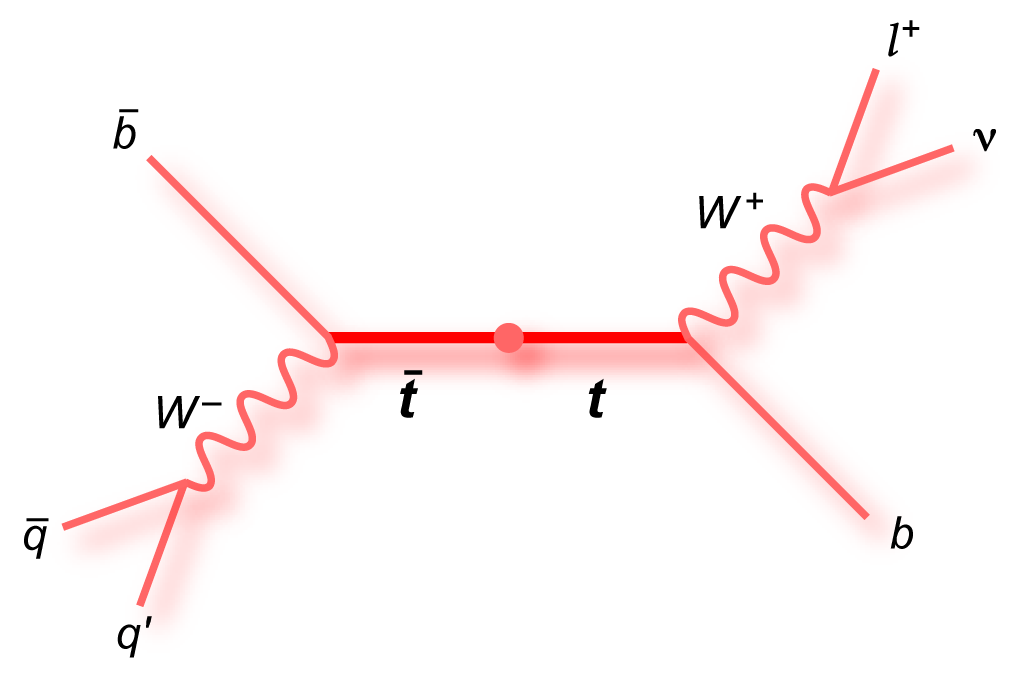
\includegraphics[width=0.4\textwidth]{figs/feynman_ttbar_ljets_beamline.png}
\caption[A diagram of a semi-leptonic $t\bar{t}$ event in the center-of-mass frame.]{A diagram of a semi-leptonic $t\bar{t}$ event in the center-of-mass frame \cite{ttbar}.}
\label{fig:ttbar}
\end{figure}

Semi-leptonic $t\bar{t}$ events, as in Figure~\ref{fig:ttbar}, are selected by requiring a single muon ($p_{T}>50\,\textrm{GeV}$, $|\eta|<2.1$) within close proximity ($\Delta\phi<\frac{2}{3}\pi$) of a loose-b-tagged AK4 jet ($p_{T}>30\,\textrm{GeV}$, $|\eta|<2.4$). Opposite this muon ($\Delta\phi>\frac{2}{3}\pi$) we require at least one AK8 jet ($p_{T}>250\,\textrm{GeV}$, $|\eta|<2.4$) and at least one AK4 jet. The AK8 jet is to be reconstructed as the W boson. Events are triggered in data by requiring a $p_{T}>50\,\textrm{GeV}$ muon at HLT. Three additional selections are applied to ensure a high purity sample:

\begin{itemize}
\item
The AK8 jet must be consistent with having a two-jet substructure (using a quantity called ``n-subjettiness'' \cite{njet1, njet2}).
\item
The AK8 jet must have a mass within the window [50, 200 GeV]. Jets from QCD tend to have low mass.
\item
To minimize contamination from nearby objects, no AK4 jets are allowed with $\Delta R<0.8$ of the reconstructed W. 
\end{itemize}

The purity of the sample can be seen on the left in Figure~\ref{fig:dists}, a plot of the AK8 jet mass - the distribution is centered near $m_{W} = 80.385\,\textrm{GeV}$. A small contribution near $m_{top}=172.44\,\textrm{GeV}$ arises from the merging of a W and b quark into a single AK8 jet.

\begin{figure}[hbp!]
\centering
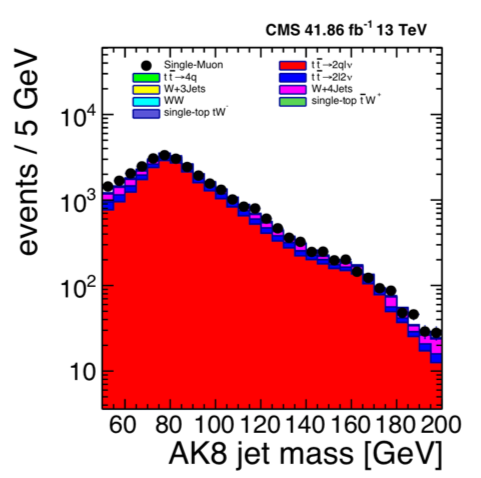
\includegraphics[width=0.465\textwidth]{figs/ak8jetmass.png}
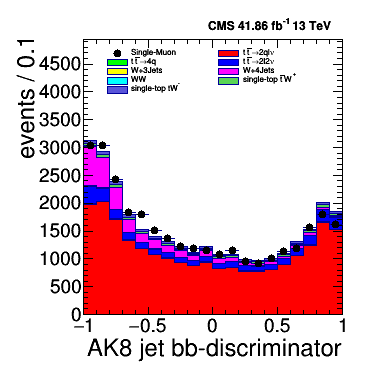
\includegraphics[width=0.48\textwidth]{figs/ak8jetbbdisc.png}
\caption{W jet mass and $b\bar{b}$-tagging discriminator in data and simulation. Simulation is scaled to match the data normalization.}
\label{fig:dists}
\end{figure}

The right side of Figure~\ref{fig:dists} shows the distribution of the $b\bar{b}$-tagging discriminator for data and simulation. For a given working point (i.e. a fixed point along the x-axis of the figure), the mistag rate in  $t\bar{t}$ MC (inclusive in all decays) is defined as the number of jets with a discriminator greater than that value, divided by the total number of jets. In data, the observed yields are first corrected by a subtraction of the expected prompt W and single-top background estimated from simulation. Equation~\ref{eq:mistags} summarizes these equations:

\begin{equation}
\label{eq:mistags}
\epsilon_{mc} = \frac{ N_{b\bar{b}-tagged}^{sig, mc} } { N^{sig, mc} }, \hspace{1cm}
\epsilon_{data} = \frac{N_{b\bar{b}-tagged}^{data}-N_{b\bar{b}-tagged}^{bkg, mc}}{N^{data} - N^{bkg, mc}}, \hspace{1cm}
\textrm{scale factor} = \frac{\epsilon_{data}} {\epsilon_{mc}}
\end{equation}

Following this prescription, we obtain the mistag rates in data and simulation seen in Table~\ref{tab:mistag}. Four working points are defined ranging from disc$>$0.3 to disc$>$0.9. It is seen that the mistag rate in MC is higher for all working points than in data. This trend can be seen in the right-hand plot of Figure~\ref{fig:dists} - the MC under-predicts the yields with low discriminator value, and over-predicts those with a large discriminator value.

\begin{table}[hbp!]
\centering
\caption{W jet $b\bar{b}$ mistag rates in data and simulation, inclusive in $p_{T}$. Errors are statistical only.}
\label{tab:mistag}
\begin{tabular}{c|cc}
\hline\hline
working point & data & MC\\
\hline
disc $>$ 0.3 & 0.326 $\pm$ 0.003 & 0.340 $\pm$ 0.003 \\
disc $>$ 0.6 & 0.219 $\pm$ 0.003 & 0.236 $\pm$ 0.002 \\
disc $>$ 0.8 & 0.122 $\pm$ 0.002 & 0.138 $\pm$ 0.002 \\
disc $>$ 0.9 & 0.058 $\pm$ 0.001 & 0.067 $\pm$ 0.001 \\
\hline\hline
\end{tabular}
\end{table}

The scale factors are then formed by taking the ratio of the mistag rate in data to that of simulation. Table~\ref{tab:sf} shows the scale factors, binned in jet $p_{T}$, for the four different working points. The errors shown arise from the quadrature sum of the statistical and two additional systematic errors: uncertainty in the normalization of the prompt-W background MC, and the effect of reweighting the $t\bar{t}$ MC to better match the top $p_{T}$ spectra observed in data \cite{toppt}. The size of the error from the prompt-W MC normalization is estimated by scaling the MC $\pm30\%$, we assign an absolute 2, 4, 6\% uncertainties for the low, medium, and high $p_{T}$ bins, respectively. The error due to the top $p_{T}$ re-weighting is estimated by taking the difference in scale factors with and without the weights. We assign an absolute error of 0, 1, 2\% to the low, medium, and high $p_{T}$ bins, respectively.

\begin{table}[hbp!]
\centering
\caption{Summary of scale factors for $b\bar{b}$-tagging W jets in $t\bar{t}$ events.}
\label{tab:sf}
\begin{tabular}{c|ccc}
\hline\hline
working point & $250 < p_{T} < 350\,\textrm{GeV}$ & $350 < p_{T} < 430\,\textrm{GeV}$ & $p_{T}>430\,\textrm{GeV}$\\
\hline
disc $>$ 0.3 & 0.939$\pm$0.026 & 1.007$\pm$0.055 & 0.996$\pm$0.079 \\
disc $>$ 0.6 & 0.922$\pm$0.027 & 0.967$\pm$0.057 & 0.902$\pm$0.082  \\
disc $>$ 0.8 & 0.875$\pm$0.030 & 0.939$\pm$0.063 & 0.893$\pm$0.090  \\
disc $>$ 0.9 & 0.855$\pm$0.036 & \multicolumn{2}{c}{0.914$\pm$0.068} \\
\hline\hline
\end{tabular}
\end{table}
